\section{Results}
\subsection{Resolution and exact forward dynamics}
Under the declared grid criterion, the seed-7 encoded target has one significant maximum for $j\leq2$ and two starting at $j=5/2$ (Fig.~\ref{fig:physics}). This motivates dimension six for the training diagnosis; it is not a universal threshold for resolving two spherical modes. Encoding and readout smooth the particular data through Eq.~\eqref{eq:kernel}.

Across all 70 diagnostic and hybrid runs, a fresh coefficient audit gives a maximum absolute forward-decay error of \AuditDecay. Saved forward and reverse states have maximum trace residual \AuditTrace, maximum Hermiticity residual \AuditHerm, and minimum eigenvalue \AuditMinEigen. Replaying the stored parameters reproduces the saved generated states to the precision reported in the audit; the maximum Kraus-completeness residual is \AuditKraus. These are numerical consistency checks, not a substitute for the analytic CPTP argument.

\begin{figure}[tbp]
 \centering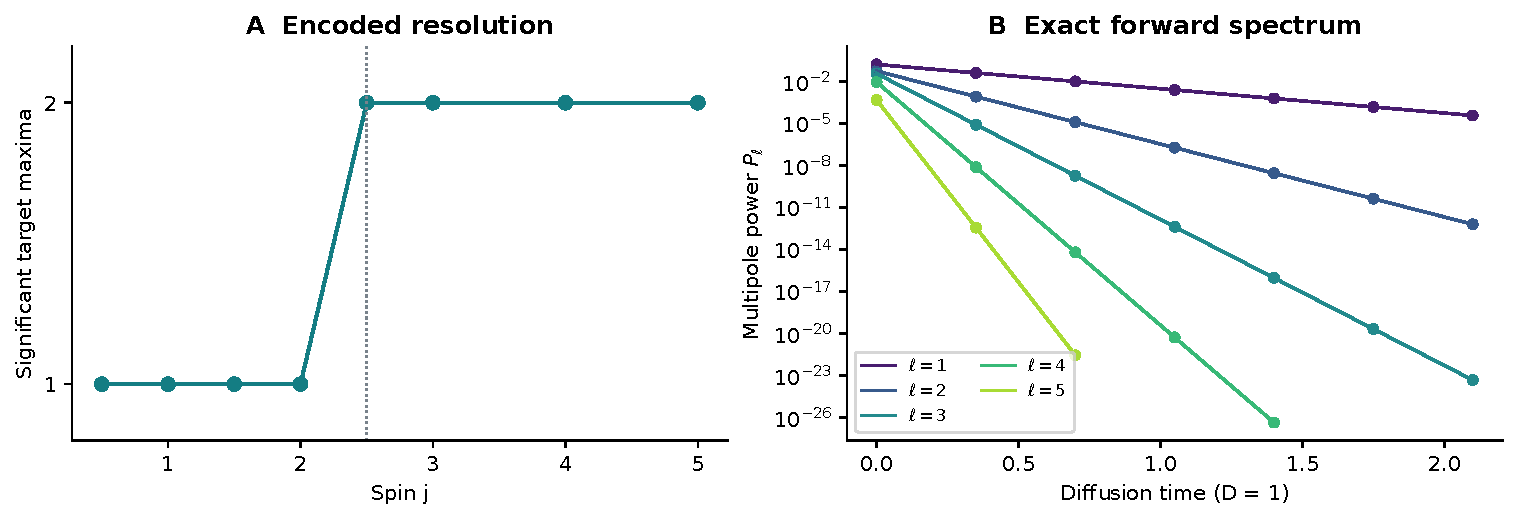
\includegraphics[width=\linewidth]{figures/physics.pdf}
 \caption{Finite resolution and forward diffusion. Left: significant maxima in the encoded target for the fixed seed-7 dataset. Right: measured multipole powers (markers) and the exact decay law (lines), using the seed-7 $j=5/2$ forward trajectory. Values below $10^{-28}$ are omitted from the logarithmic plot because floating-point residuals dominate. All retained ranks are present in the saved data.}
 \label{fig:physics}
\end{figure}

\subsection{Final supervision resolves the missing-mode failure}
Table~\ref{tab:diagnostic} reports every condition in the paired 40-run diagnostic. At 100 epochs, fidelity path supervision recovers both modes in one of five seeds for either start. Final-only supervision recovers both in all five. For the generative mixed prior, mean infidelity falls from approximately $4.21\times10^{-2}$ to $7.17\times10^{-4}$ and mean trace distance from $0.1328$ to $0.0161$. Switching to the exact terminal forward state does not remove the path-training failure.

\begin{table}[tbp]
 \centering\small
 \caption{Controlled diagnostic at $j=5/2$. Each row summarizes the same five seeds. Entries are mean $\pm$ sample standard deviation; mode counts are successes out of five. $\rho_6$ is the target-dependent terminal forward state.}
 \label{tab:diagnostic}
 \begin{tabular}{lllcrr}
\toprule
Start & Loss & Epochs & Modes & Infidelity & Trace distance \\
\midrule
$\id/d$ & path & 100 & 1/5 & $0.0421\pm0.0132$ & $0.1328\pm0.0257$ \\
$\id/d$ & final & 100 & 5/5 & $(7.17\pm3.73)\,10^{-4}$ & $0.0161\pm0.0059$ \\
$\rho_6$ & path & 100 & 1/5 & $0.0422\pm0.0121$ & $0.1334\pm0.0234$ \\
$\rho_6$ & final & 100 & 5/5 & $(8.35\pm4.46)\,10^{-4}$ & $0.0176\pm0.0067$ \\
$\id/d$ & path & 500 & 5/5 & $0.0122\pm0.0011$ & $0.0690\pm0.0062$ \\
$\id/d$ & final & 500 & 5/5 & $(2.98\pm2.26)\,10^{-5}$ & $(3.05\pm0.62)\,10^{-3}$ \\
$\rho_6$ & path & 500 & 5/5 & $0.0112\pm0.0007$ & $0.0650\pm0.0059$ \\
$\rho_6$ & final & 500 & 5/5 & $(2.70\pm1.16)\,10^{-5}$ & $(3.12\pm1.13)\,10^{-3}$ \\
\bottomrule
\end{tabular}

\end{table}

At 500 epochs, all four conditions recover both modes, but the final-only objective retains substantially lower state error. Rank-resolved errors likewise reveal structure missed by global visual similarity (Fig.~\ref{fig:diagnostic}). In the original 100-epoch mixed-prior path runs, correlations of the generated and target Husimi grids exceed $0.995$ even in failures. High correlation alone is therefore insufficient evidence of multimodal recovery.

\begin{figure}[tbp]
 \centering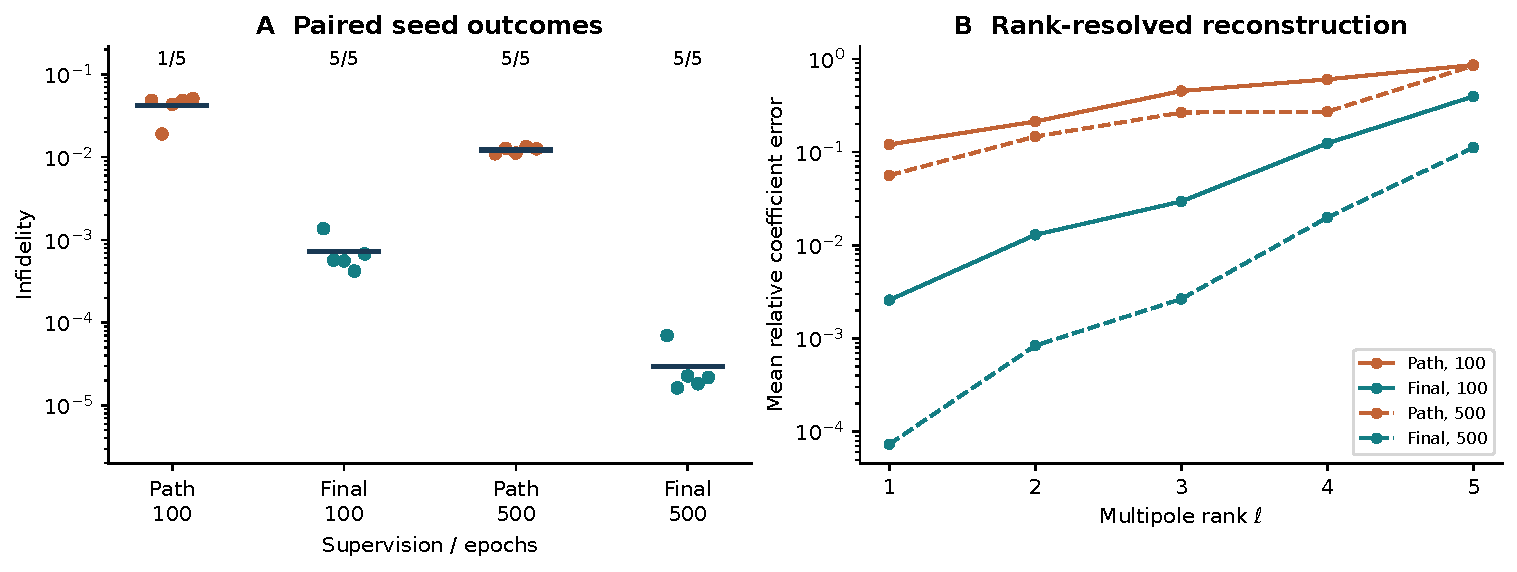
\includegraphics[width=\linewidth]{figures/diagnostic.pdf}
 \caption{Training diagnosis for the generative mixed prior. Left: individual-seed infidelity and group means for the two objectives and epoch budgets; annotations give both-mode recovery. Right: mean relative coefficient error by rank, retaining phase and orientation information. Each curve aggregates the same five seeds. These are descriptive paired experiments; the figure does not isolate a unique optimization mechanism.}
 \label{fig:diagnostic}
\end{figure}

These results show that the fixed architecture can represent a successful generated state for this problem. They support the supervision choice and optimization budget as practical limitations of the original run. They do not establish a general superiority of final-only objectives: scale normalization, alternative learning rates, and intermediate-state gradient interactions were not separately controlled. Moreover, final-only training uses no intermediate forward targets; its success is also consistent with a deep dissipative state-preparation model.

\subsection{Validation-selected multipole weighting improves high-rank accuracy}
The saved selection rule chooses $\lambda=0.75$. Both the selected hybrid and pure fidelity recover both modes for all five confirmation seeds. Table~\ref{tab:hybrid} shows all validation candidates and both confirmation conditions. On confirmation, mean $E_{45}$ decreases from $1.4272\times10^{-5}$ to $2.8103\times10^{-6}$, a \HybridRankReduction\% reduction. Mean trace distance falls by \HybridTraceReduction\%, from $0.003612$ to $0.001767$. The mean JS divergence increases by approximately $7.48\times10^{-8}$, within the predeclared absolute guardrail. Thus the improvement concerns reconstruction accuracy rather than the already saturated binary mode count.

\begin{table}[tbp]
 \centering\small
 \caption{Hybrid selection and confirmation. Each row contains five seeds; all rows recover both modes in five of five runs. Entries are means, with per-seed values and uncertainty in the archive. $E_{45}$ is the squared error of rank-4 and rank-5 coefficients. Confirmation seeds were not used to choose $\lambda$.}
 \label{tab:hybrid}
 \begin{tabular}{llrrrr}
\toprule
Split & $\lambda$ & Infidelity & Trace distance & JS (nats) & $E_{45}$ \\
\midrule
Validation & 0 & $3.28\times10^{-5}$ & $3.48\times10^{-3}$ & $9.35\times10^{-7}$ & $1.54\times10^{-5}$ \\
Validation & 0.25 & $3.57\times10^{-5}$ & $3.18\times10^{-3}$ & $1.08\times10^{-6}$ & $1.24\times10^{-5}$ \\
Validation & 0.5 & $2.83\times10^{-5}$ & $2.20\times10^{-3}$ & $7.78\times10^{-7}$ & $4.92\times10^{-6}$ \\
Validation & 0.75 & $3.33\times10^{-5}$ & $1.75\times10^{-3}$ & $8.37\times10^{-7}$ & $2.59\times10^{-6}$ \\
Confirmation & 0 & $3.52\times10^{-5}$ & $3.61\times10^{-3}$ & $1.02\times10^{-6}$ & $1.43\times10^{-5}$ \\
Confirmation & 0.75 & $2.96\times10^{-5}$ & $1.77\times10^{-3}$ & $1.10\times10^{-6}$ & $2.81\times10^{-6}$ \\
\bottomrule
\end{tabular}

\end{table}
\begin{figure}[tbp]
 \centering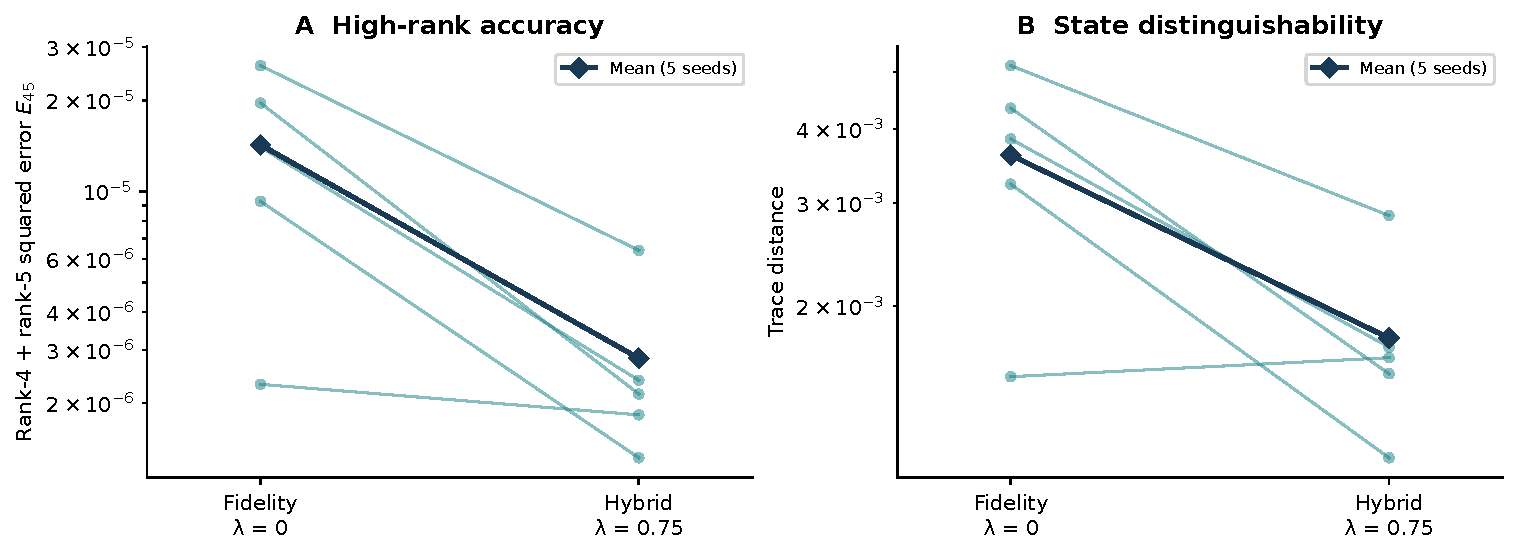
\includegraphics[width=\linewidth]{figures/hybrid.pdf}
 \caption{Paired confirmation outcomes at 500 epochs. Lines connect the same seed under pure fidelity and the selected hybrid; dark markers give the group means. The reduction in the means does not imply improvement on every individual seed. Axes are logarithmic to show relative differences.}
 \label{fig:hybrid}
\end{figure}

\subsection{Instrument consistency and the correlated-model limitation}
The historical instrument study applies ancilla measurements to the five original 100-epoch $j=5/2$ fidelity models, using 256 trajectories per model. The mean squared Frobenius distance between the trajectory ensemble and deterministic channel output is $0.000701\pm0.000279$, and the mean trace distance is $0.02466\pm0.00540$. These sample fluctuations are compatible with the exact branch-average identity. They do not constitute a demonstrated sampling-speed benefit. The archive contains the aggregate instrument tables; individual conditional trajectories were not retained, so these ensemble values are preserved historical results rather than a fresh trajectory-level audit.

The independent test state in the two-spin pilot has quantum mutual information $0.34454$ nats. The factorized baseline loses this dependence, but both learned quantum models are less accurate even than that baseline in trace distance (Table~\ref{tab:two}). Direct interactions improve the quantum results slightly; they do not close the much larger gap to the spherical kernel, separable mixture, or neural generator. The six saved model states pass a fresh independent metric comparison with maximum discrepancy \AuditTwoDelta.

\begin{table}[tbp]
 \centering\small
 \caption{Two-spin pilot, one independent train/test split. Parameter counts distinguish trainable (t) from effective (e) counts. Errors compare to the same encoded test state; MI is quantum mutual information in nats. Different training budgets and objectives preclude a resource-matched advantage claim.}
 \label{tab:two}
 \begin{tabular}{lrrrr}
\toprule
Model & Parameters & Trace dist. & MI error & Corr. error \\
\midrule
Factorized marginals & 16 e & 0.3272 & 0.3445 & 0.4525 \\
Spherical kernel & 0 t & 0.0342 & 0.0139 & 0.0157 \\
Separable mixture & 33 e & 0.0405 & 0.0468 & 0.0391 \\
Quantum, no direct & 33 t & 0.5328 & 0.3253 & 0.4849 \\
Quantum, direct & 39 t & 0.5286 & 0.3195 & 0.4623 \\
Neural generator & 39 t & 0.0526 & 0.0431 & 0.0324 \\
\bottomrule
\end{tabular}

\end{table}
The two-spin experiment therefore establishes an implemented correlated extension and a baseline comparison, not successful competitive many-body generation. It also cannot attribute a role to entanglement: the target encoding is separable and no entanglement ablation was performed.
